\chapter{飛行ロボコン}

\section{大会ルール}
ヘリポートから飛行を開始し,ミッションエリアにてミッションを完了したのち,ヘリポートに帰還する.
大会のフィールドを図2.1に示す.

\begin{figure}[htbp]
  \begin{center}
    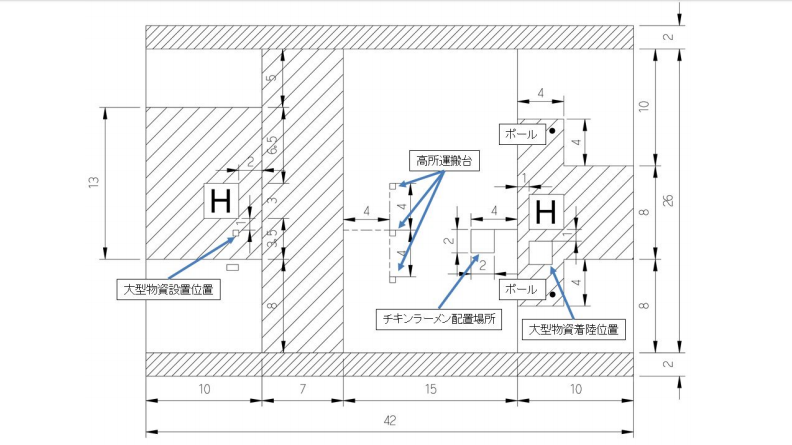
\includegraphics[width=120mm]{img/フィールド.jpg}
    \end{center}
  \caption{大会フィールド}
 \label{fig:robot}
\end{figure}

\section{機体条件}
大会に出場するための機体には以下の条件を満たさないといけない.
\begin{enumerate}
  \item 空虚重量が350g以下であり,地上補助装置との合計重量が500g以下である.
  \item 機体は自作である.
  \item 推進力として2つ以上のプロペラを搭載する機体である.
  \item 搭載する全てのプロペラ周りに安全のためにプロペラガードなどを取り付けること.

\end{enumerate}

大会に出場した機体を図2.2に示す.

\begin{figure}[htbp]
  \begin{center}
    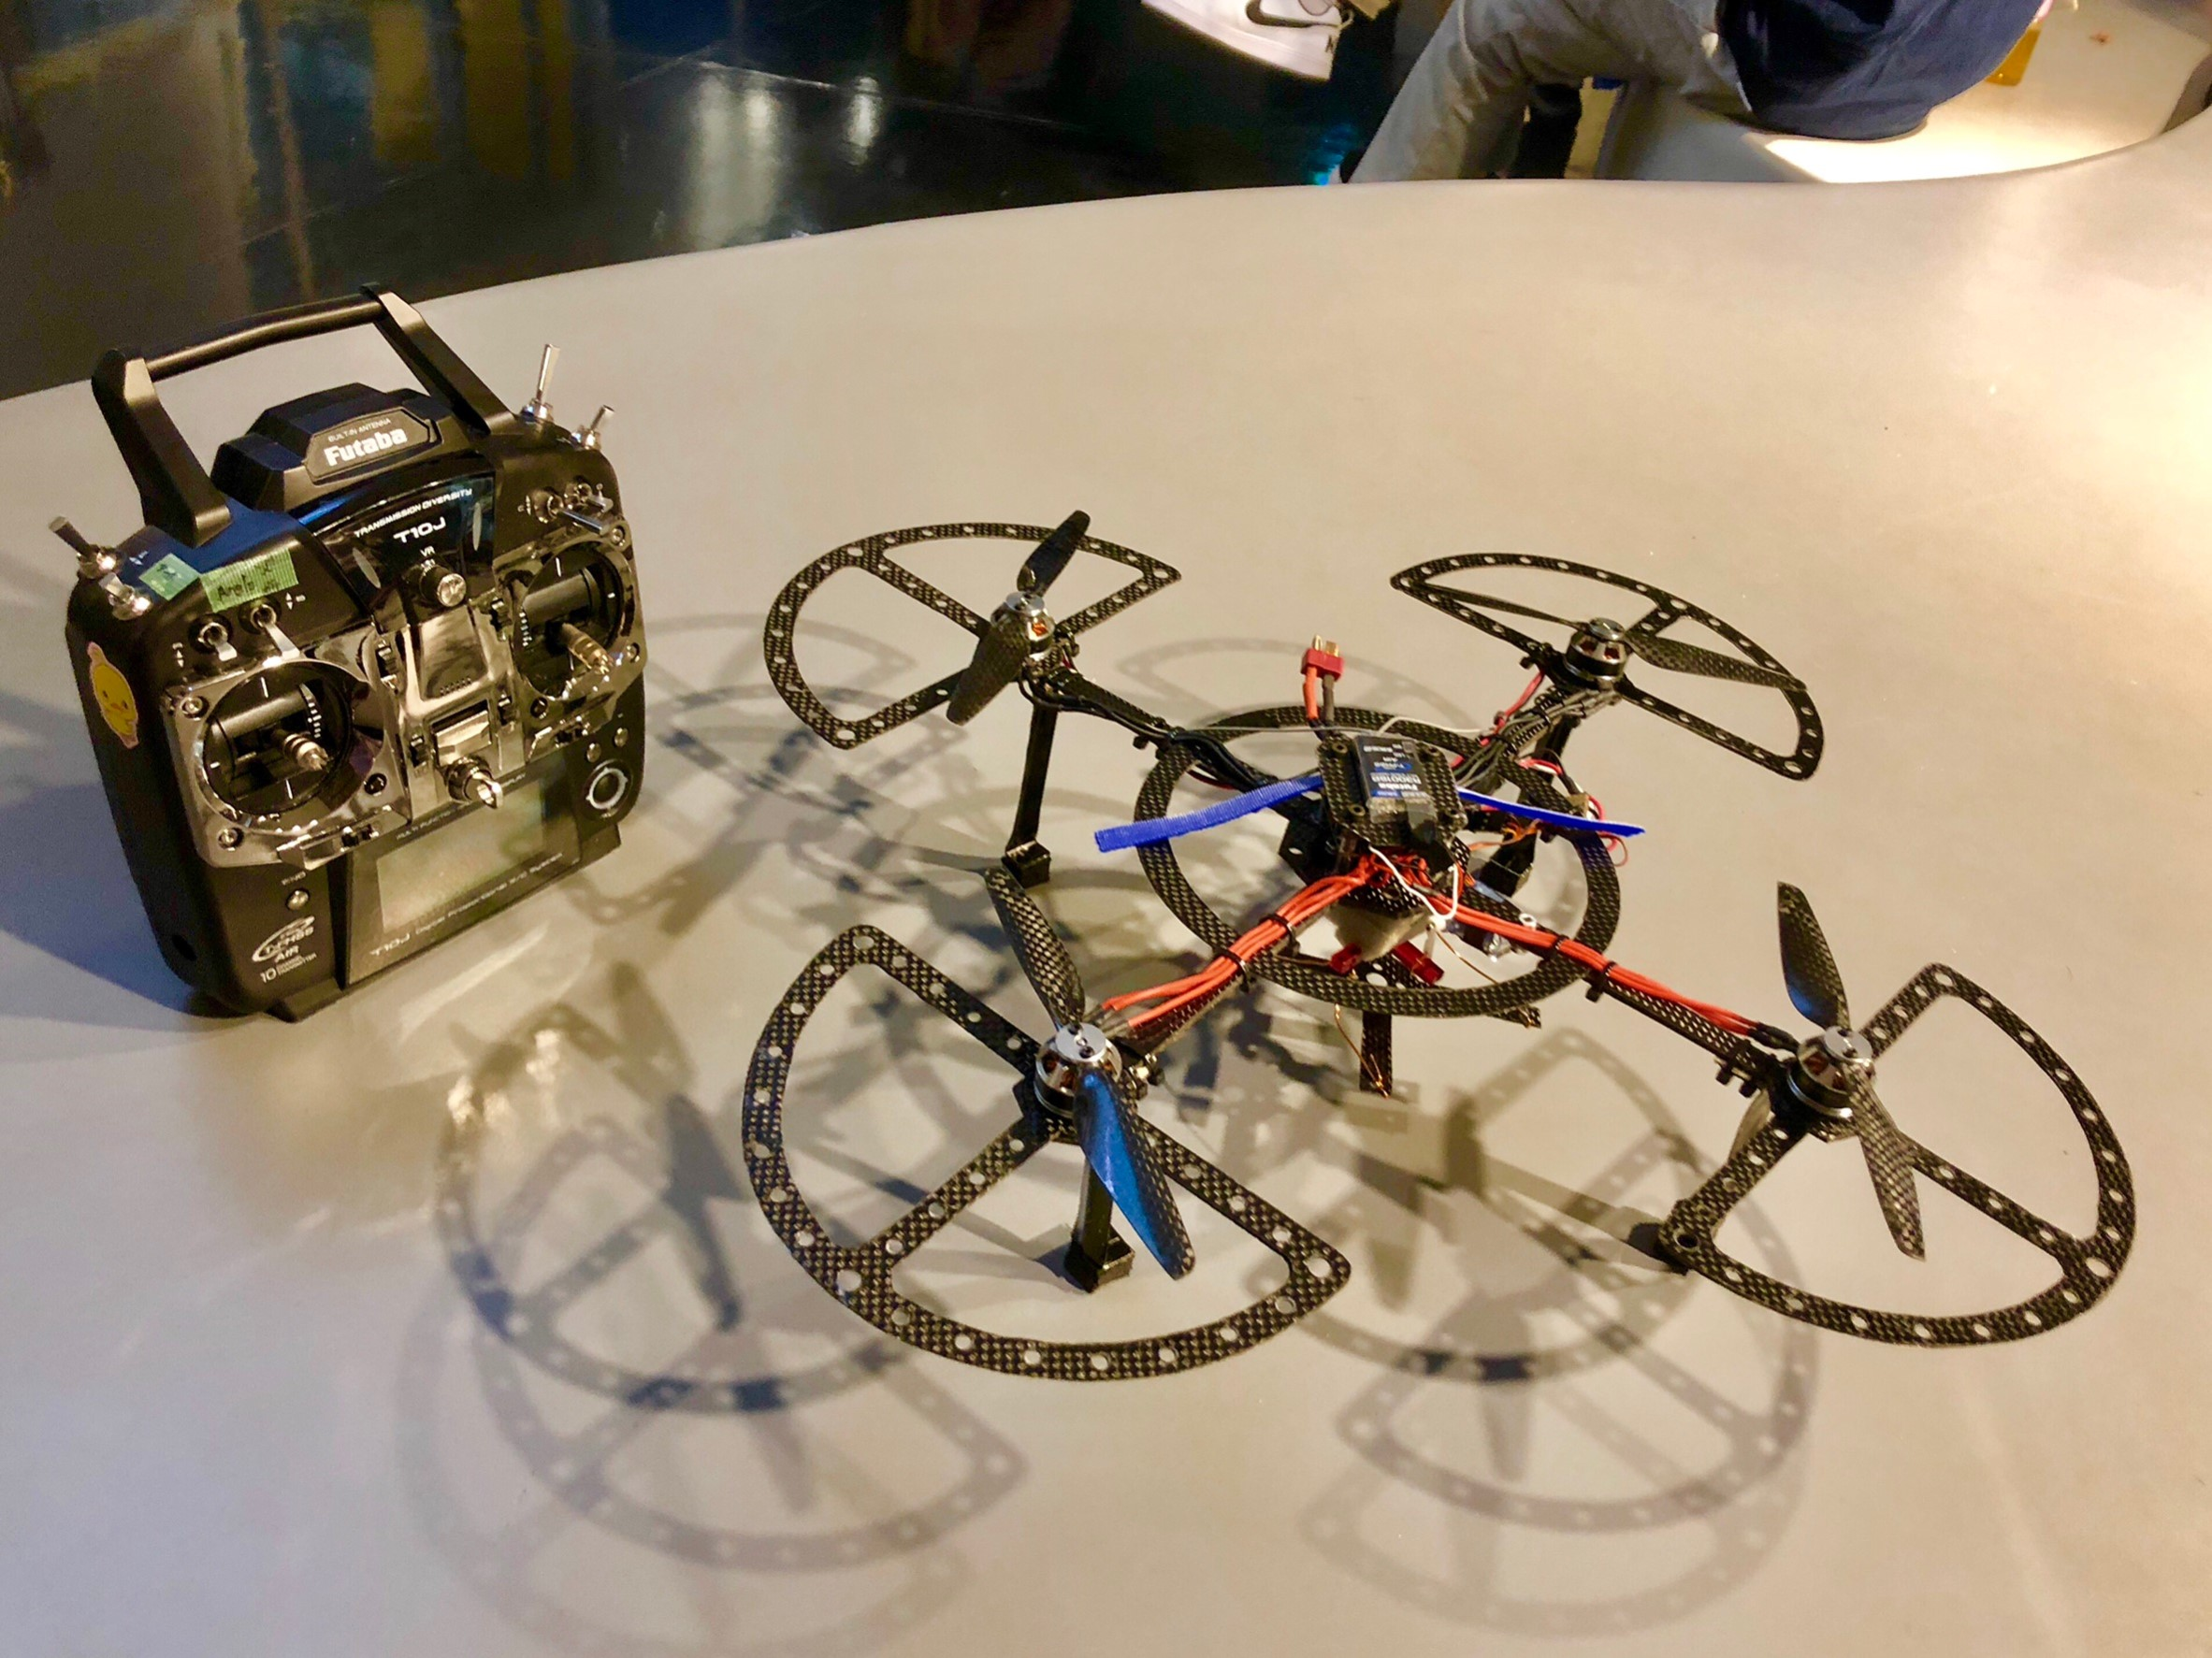
\includegraphics[width=100mm]{img/大会機.JPG}
    \end{center}
  \caption{大会機}
 \label{fig:robot}
\end{figure}

\def\MARU#1{{\rm\ooalign{\hfil\lower.168ex\hbox{#1}\hfil \crcr\mathhexbox20D}}}

我々の機体の特徴を以下に示す.
\begin{enumerate}
  \item カーボンシートを積層し軽量化かつ高い強度が得られるよう計った.カーボンを使用することで大会出場条件の350g以下になっている.
  \item 前後の進行方向の区別を目視しやすくするためにピンク色のLEDランプを使用した.そのため操縦士から見やすくなり容易に操縦できるようになる.
  \item 高所物資運搬のミッションで箱の中身を確認するのに超小型の動画撮影用のカメラを使用した.このカメラを使うことで,箱の中身を確認した後に元の位置に戻る手間が無線じゃないため電波障害が起きることがない.
  \item 操縦士がより機体を操縦できるように,機体の揺れを少なく制御を行った.
\end{enumerate}


\section{ミッション}
マルチコプター部門のミッションは以下の5種類で,\MARU{1}のミッションは競技開始と同時に開始される.\MARU{1}のミッションが終了した後,\MARU{2}~\MARU{4}のミッションの順番は問わない.\MARU{5}は最後に行うこと.

\MARU{1} 「高所物資運搬」,\MARU{2} 「大型物資運搬」,\MARU{3} 「Rocking Wings」,\MARU{4}「8の字飛行」,\MARU{5}「自動離着陸」

予選と決勝におけるミッション
予選では「高所物資運搬」「8の字飛行」の2つのみ挑戦をが認められる.決勝では全てのミッションへの挑戦が認められる.

\section{大会結果}
大会は11チーム出場し,我々の予選結果は840点を獲得し2位となり決勝へと駒を進めた.
決勝は4チーム勝ち上がった.
決勝で我々が挑戦したミッションは予選の「高所物資運搬」と「8の字飛行」に加えて,「大型物資運搬」に挑戦した.
3つのミッションに挑戦した結果,1925点獲得し2位と500点近くの差をつけて優勝することができた.

\section{大会の勝因}

我々の大会の勝因を以下に示す.
\begin{enumerate}
  \item フレームすべてをカーボンにしたことで軽量で高い強度が得られた.またフレームの厚みを変えたことで軽くなった.
  \item 高所物資運搬のミッションにチキンラーメンを箱の中に入れるためのサーボ機構が安定していた.そのため機体に与える影響が少なくなった.
  \item 戦略がよく高得点が出た.自動を含むミッションに挑戦しなかったため電波障害が起きることがなかった.
  \item 制御の安定性があったため機体の揺れが少なく,操縦しやすくなっていた. 
  \item 操縦士の技量があり,緊張もせずに挑むことができた.
\end{enumerate}

\section{大会の反省点}

我々の大会の反省点を以下に示す.
\begin{enumerate}
  \item 大会ルールの確認不足.大会で使用できるバッテリーのセル数は2セルなのだが確認不足だったため3セルで出場しようとしてしまい,会場の近くのお店に急いで買い出しに行くこととなった.
  \item 大会前の準備期間のスケジュールがチーム内で全員が揃うことが少なかった.
\end{enumerate}






